% !TeX root = ../index.tex
\chapter{Database Connectivity \& Functions}
\graphicspath{{6-db-functions/images/}}

\section{Exercise 1}

\url{https://intweb.bucks.ac.uk/~21606555/oos/6-db-functions/ex1.html}

\captionsetup{type=figure}\captionof{figure}{ex1.html}
\subfile{pyg/src/6-db-functions/ex1}

\clearpage
\captionsetup{type=figure}\captionof{figure}{ex1-action.php}
\subfile{pyg/src/6-db-functions/ex1-action}

\begin{figure}[H]
  \caption{Exercise 1 - Result}
  \centering
  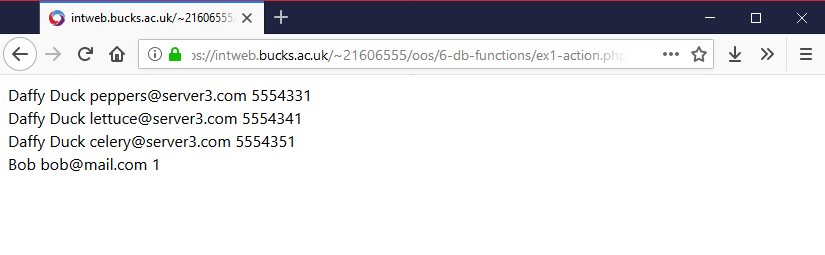
\includegraphics[width=\textwidth]{ex1}
\end{figure}

\clearpage
\section{Exercise 2}

\url{https://intweb.bucks.ac.uk/~21606555/oos/6-db-functions/ex2.php}

\captionsetup{type=figure}\captionof{figure}{ex2.php}
\subfile{pyg/src/6-db-functions/ex2}

\clearpage
\captionsetup{type=figure}\captionof{figure}{ex2-action.php}
\subfile{pyg/src/6-db-functions/ex2-action}

\begin{figure}[H]
  \caption{Exercise 2 - List of users}
  \centering
  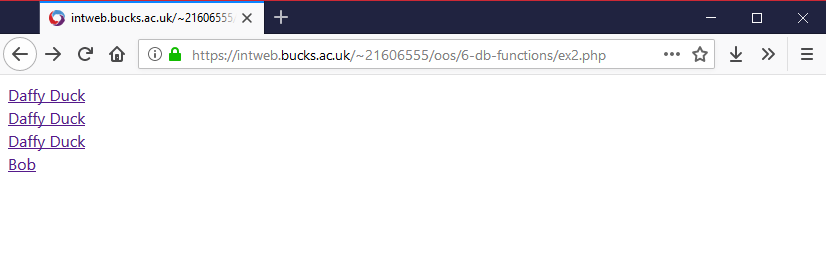
\includegraphics[width=\textwidth]{ex2-1list}
\end{figure}

\begin{figure}[H]
  \caption{Exercise 2 - Editing a user}
  \centering
  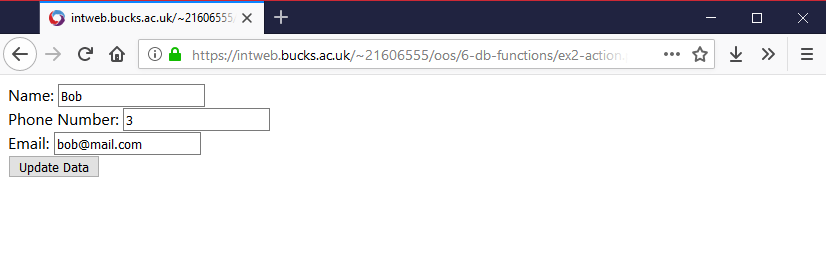
\includegraphics[width=\textwidth]{ex2-2edit}
\end{figure}

\clearpage
\section{Exercise 3}

\captionsetup{type=figure}\captionof{figure}{ex3-action.php}
\subfile{pyg/src/6-db-functions/ex3-action}

\begin{figure}[H]
  \caption{Exercise 3 - Updated the user from exercise 2}
  \centering
  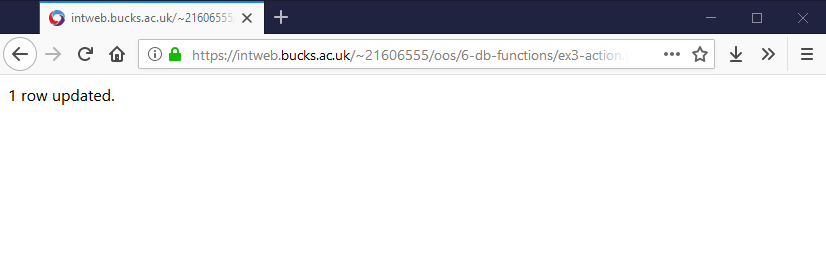
\includegraphics[width=\textwidth]{ex3-1update}
\end{figure}

\begin{figure}[H]
  \caption{Exercise 3 - User data has been updated}
  \centering
  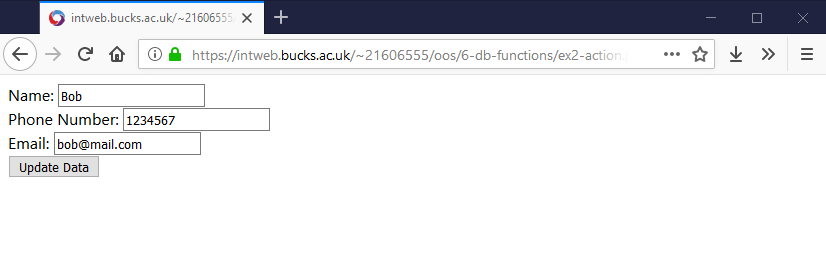
\includegraphics[width=\textwidth]{ex3-2result}
\end{figure}

\clearpage
\section{Exercise 4}

\captionsetup{type=figure}\captionof{figure}{ex4-action.php}
\subfile{pyg/src/6-db-functions/ex4-action}

\begin{figure}[H]
  \caption{Exercise 4 - Ability to delete users}
  \centering
  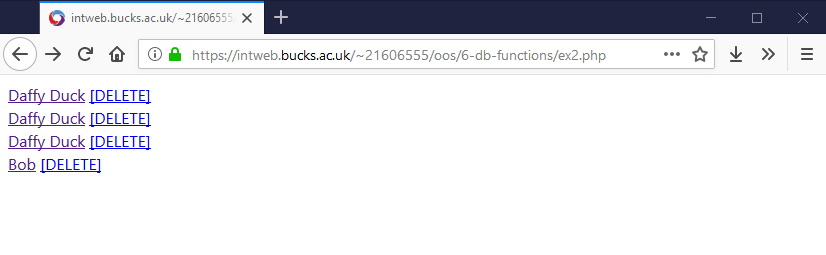
\includegraphics[width=\textwidth]{ex4-1list}
\end{figure}

\begin{figure}[H]
  \caption{Exercise 4 - Deleting a user}
  \centering
  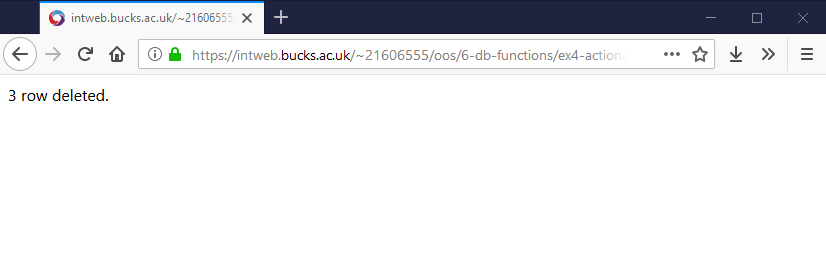
\includegraphics[width=\textwidth]{ex4-2delete}
\end{figure}

\begin{figure}[H]
  \caption{Exercise 4 - List without deleted users}
  \centering
  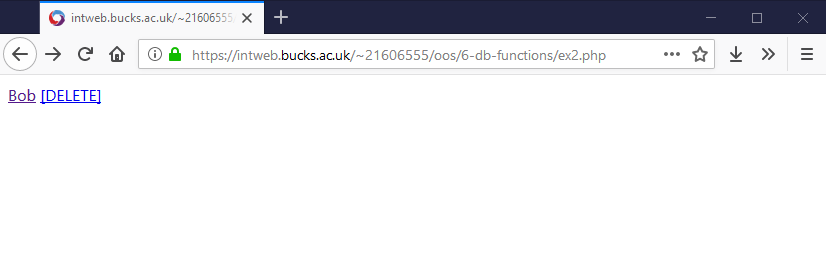
\includegraphics[width=\textwidth]{ex4-3result}
\end{figure}

\clearpage
\section{Exercise 5}

\url{https://intweb.bucks.ac.uk/~21606555/oos/6-db-functions/ex5.php}

\captionsetup{type=figure}\captionof{figure}{ex5-functions.php}
\subfile{pyg/src/6-db-functions/ex5-functions}

\captionsetup{type=figure}\captionof{figure}{ex5.php}
\subfile{pyg/src/6-db-functions/ex5}

\begin{figure}[H]
  \caption{Exercise 5 - Output}
  \centering
  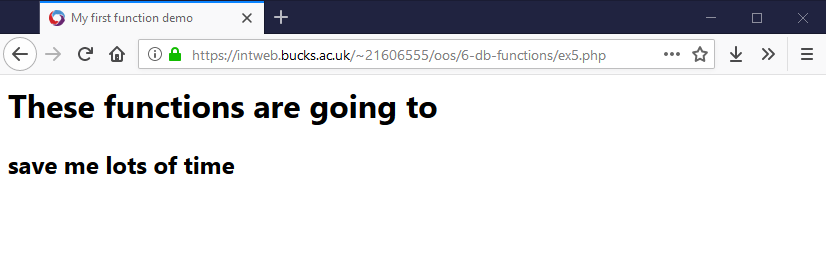
\includegraphics[width=\textwidth]{ex5}
\end{figure}

\clearpage
\section{Exercise 6}

\url{https://intweb.bucks.ac.uk/~21606555/oos/6-db-functions/ex6.php}

\captionsetup{type=figure}\captionof{figure}{ex6-functions.php}
\subfile{pyg/src/6-db-functions/ex6-functions}

\captionsetup{type=figure}\captionof{figure}{ex6.php}
\subfile{pyg/src/6-db-functions/ex6}

\begin{figure}[H]
  \caption{Exercise 6 - Output}
  \centering
  
\includegraphics[width=\textwidth]{ex6}
\end{figure}

\clearpage
\section{Exercise 7}

\url{https://intweb.bucks.ac.uk/~21606555/oos/6-db-functions/ex7.php}

\captionsetup{type=figure}\captionof{figure}{ex7-functions.php}
\subfile{pyg/src/6-db-functions/ex7-functions}

\captionsetup{type=figure}\captionof{figure}{ex7.php}
\subfile{pyg/src/6-db-functions/ex7}

\begin{figure}[H]
  \caption{Exercise 7 - Output}
  \centering
  \includegraphics[width=\textwidth]{ex7}
\end{figure}

\clearpage
\section{Exercise 8}

\url{https://intweb.bucks.ac.uk/~21606555/oos/6-db-functions/ex8.php}

\captionsetup{type=figure}\captionof{figure}{ex8-functions.php}
\subfile{pyg/src/6-db-functions/ex8-functions}

\captionsetup{type=figure}\captionof{figure}{ex8.php}
\subfile{pyg/src/6-db-functions/ex8}

\begin{figure}[H]
  \caption{Exercise 8 - Output}
  \centering
  \includegraphics[width=\textwidth]{ex8}
\end{figure}
